\documentclass{../templates/topic}

\begin{document}
\graphicspath{{assets/}{ch2a_Transfer_Functions/assets/}}

\chapter{Transfer Functions}

\begin{section}{Definition}
	The transfer function is defined as:
	\begin{equation}
		G(s) = \frac{\laplace[Output]}{\laplace[Input]}
	\end{equation}
	
	For a system defined as $\{a_{n}*D_{n}[y] \} = \{b_{m}*D_{m}[x] \}$ where y is the output and x is the input, the transfer function is given as:
	
	\begin{equation}
		G(s) = \frac{Y(s)}{X(s)} = \frac{\{a_{n}*s^{n}\}}{\{b_{m}*s^{m}\}}
	\end{equation}
	
	Note that the transfer function is not unique; there are many systems which reduce to the same transfer function.
	Note also that the transfer function is not tied to the input function.
	The transfer function does not provide information about the physical system underlying the model, and many different systems with different physical quantities being studied can have the same transfer function.
	The transfer function is limited to linear, time-invariant differential equations.
	
\end{section}

\begin{section}{TF of a Closed-Loop System}
	
	For a general closed-loop system, there are several transfer functions of interest.
	
	\begin{figure}[H]
		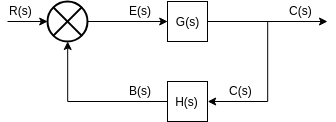
\includegraphics[width=\textwidth]{closed_loop.png}
		\caption{General Closed-Loop system block diagram}
	\end{figure}
	
	\definition{Closed-Loop} $\frac{C(s)}{R(s)}=\frac{G(s)}{1+G(s)H(s)}$
	
	\definition{Feed-Forward} $\frac{C(s)}{E(s)}=G(s)$
	
	\definition{Error Ratio} $\frac{E(s)}{R(s)}=\frac{1}{1-G(s)H(s)}$
	
\end{section}

\end{document}
